\documentclass[xcolor=table,compress,professionalfonts,pdfpagelabels]{beamer}

\usepackage[english]{babel}
\usepackage{fontenc}

\usepackage{graphicx}
\graphicspath{{figures/}{photos/}}

\usepackage{hyperref}
\mode<presentation>{
 \usetheme{WM}
}

\makeatletter
% Stuff for calc compatibility.
\let\real=\pgfmath@calc@real
\let\minof=\pgfmath@calc@minof
\let\maxof=\pgfmath@calc@maxof
\let\ratio=\pgfmath@calc@ratio
\let\widthof=\pgfmath@calc@widthof
\let\heightof=\pgfmath@calc@heightof
\let\depthof=\pgfmath@calc@depthof
\makeatother

% Title and such
\title{Physics Innovation and Entrepreneurship at a Liberal Arts University}
\subtitle{CC-BY-SA}
\author{Wouter Deconinck}
\institute{William \& Mary}
\date{AAPT Summer 2016}
\event{Physics and the Maker Movement}

% Let's get started
\begin{document}

% Physics Innovation and Entrepreneurship at a Liberal Arts University
%
% The Small Hall Makerspace in the Physics Department at the College of William & Mary, Virginia, provides students with access to equipment that is usually only found in research labs and machine shops, off-limits to all but a few. By encouraging an ecosystem of student clubs and the integration of makerspace activities in courses, the makerspace has expanded to provide students of both arts and sciences with a space where they can learn and innovate in interdisciplinary groups without the time pressures and rigid expectations of traditional teaching labs. In collaboration with the Entrepreneurship Center of the Business School, we are developing an entrepreneurship physics track that combines makerspace projects with development of funding proposals, business plans and management plans. At our relatively small institution without an engineering school we are using the makerspace to create experiences in innovation and entrepreneurship for our students


\begin{frame}[plain]
 \maketitle
\end{frame}

\begin{frame}{William \& Mary: Liberal Arts University}
 \begin{block}{Primarily undergraduate liberal arts institution}
  \begin{itemize}
   \item No large medical or engineering program
   \begin{itemize}
    \item Large service courses satisfy gen-ed and pre-med requirements
   \end{itemize}
  \end{itemize}
 \end{block}
 \begin{block}{Primarily undergraduate liberal arts institution with}
  \begin{itemize}
   \item Graduate programs in select departments with traditional strengths
    \begin{itemize}
     \item PhD programs in History, American Studies (Jamestown, Williamsburg)
     \item PhD programs in Physics, Applied Science (NASA Langley, Jefferson Lab)
     \item Masters programs in Chemistry, Computer Science, Psychology,\ldots
    \end{itemize}
   \item Education school, business school (with entrepreneurship center)
  \end{itemize}
 \end{block}
 \begin{block}{Physics department at William \& Mary}
  \begin{itemize}
   \item Approximately 30 majors and 15 graduate students each year
   \item Primary preparation for graduate school (as too many physics degrees)
   \item Desire to prepare students better for the careers that await them
  \end{itemize}
 \end{block}
\end{frame}

\begin{frame}{Careers for Physicists Primarily Outside Academia}
 \begin{block}{Bachelors degrees in physics}
  \begin{itemize}
   \item Only 1 out of 6 physicists gets a PhD degree (AIP SRC)
   \item All other physicists not included in ``traditional physicists'' interpretation
  \end{itemize}
 \end{block}
 \begin{block}{PhD degrees in physics}
  \begin{itemize}
   \item Majority of permanent jobs are outside of academia
   \item About 1700 physics PhDs per year, significantly fewer jobs in academia
   \item All other physicists not included in ``traditional physicists'' interpretation
  \end{itemize}
 \end{block}
 \begin{block}{Mismatch between curriculum and reality of physics teaching}
  \begin{itemize}
   \item How can we prepare our undergraduate and graduate students better for their most likely career?
   \item What opportunities can we provide as part of the curriculum?
   \item What opportunities can we provide outside the curriculum?
  \end{itemize}
 \end{block}
\end{frame}

\begin{frame}{Careers for Physicists Primarily Outside Academia}
 \begin{columns}[t]
  \begin{column}{0.49\textwidth}
   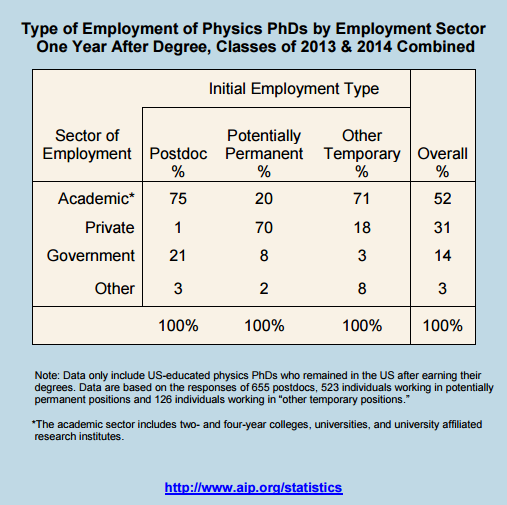
\includegraphics[width=\textwidth]{phdinitemp1}
  \end{column}
  \begin{column}{0.49\textwidth}
   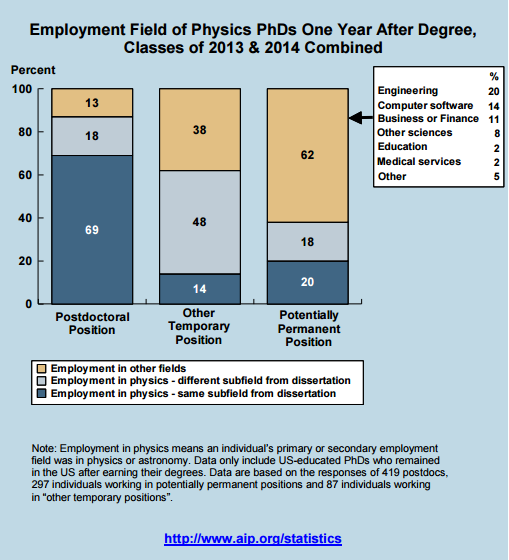
\includegraphics[width=\textwidth]{phdinitemp2}
  \end{column}
 \end{columns}
\end{frame}

\begin{frame}{Careers for Physicists Primarily Outside Academia}
 \begin{block}{What skills are physicists missing?\footnotemark}
  \begin{columns}[T]
   \begin{column}{0.5\textwidth}
    \begin{itemize}
     \item Ability to design a system, component or process to meet a specific need
     \item Ability to function on multi-disciplinary teams
     \item Ability to recognize value of diverse relationships (customers, supervisors, etc)
     \item Leadership skills
    \end{itemize}
   \end{column}
   \begin{column}{0.5\textwidth}
    \begin{itemize}
     \item Familiarity with basic business concepts (i.e. cost-benefit analysis, funding sources, IP, project management)
     \item Communication skills (oral and written), esp. how to tailor message to audience
     \item Real-world experience in companies before graduation
     \item Awareness of career paths outside of academia
    \end{itemize}
   \end{column}
  \end{columns}
 \end{block}
 \footnotetext{Sources: ABET Survey of Applied and Engineering Physics Graduates, Kettering University; APS Workshop on National Issues in Industrial Physics, Industrial Physics Lunches.}
\end{frame}

\begin{frame}{Educational Goals of the Small Hall Makerspace}
 \begin{block}{Small Hall Makerspace}
  \begin{itemize}
   \item Formed in Fall 2013 for interdisciplinary team-based projects 
   \item ``We provide the tools, students bring their creativity''
  \end{itemize}
 \end{block}
 \begin{block}{Encourage failure as fundamental to innovation}
  \begin{itemize}
   \item Instill ``fail early, fail often'' attitude
   \item No cost to failure (whether financial or to GPA) in makerspace projects
  \end{itemize}
 \end{block}
 \begin{block}{Value prototyping process over the solution itself}
  \begin{itemize}
   \item Students have strong theoretical basis but weaker practical experience
   \item Students are used to getting to ``right'' answer on straightforward path
   \item Laboratory exercises (even if self-guided and not recipe-driven) still often follow a predictable path towards a single solution
  \end{itemize}
 \end{block}
\end{frame}

\begin{frame}{Small Hall Makerspace at W\&M}
 \begin{block}{Electronics and computation workshop}
  \begin{itemize}
   \item Raspberry Pis, Intel Edison, Arduinos and many shields, Oculus Rift VR headsets
   \item Server rack (old lattice QCD nodes)
  \end{itemize}
 \end{block}
 \begin{block}{Rapid prototyping shop}
  \begin{itemize}
   \item 3D printers, laser cutters, vacuum thermoformer
   \item Actobotics and 80/20 mechanical erector set
  \end{itemize}
 \end{block}
 \begin{block}{Student machine shop}
  \begin{itemize}
   \item Drill press, milling machines, lathes
   \item 3 axis $2' \times 3'$ CNC
  \end{itemize}
 \end{block}
\end{frame}

\begin{frame}{Small Hall Makerspace at W\&M}
 \begin{block}{Rapid prototyping and electronics shop}
 \begin{center}
  \includegraphics[height=0.75\textheight]<1>{IMG_20150911_115502}
  \includegraphics[height=0.75\textheight]<2>{IMG_20150911_115512}
  \includegraphics[height=0.75\textheight]<3>{IMG_20150911_115542}
 \end{center}
 \end{block} 
\end{frame}

\begin{frame}{Small Hall Makerspace at W\&M}
 \begin{block}{Student machine shop (under supervision only)}
 \begin{center}
  \includegraphics[height=0.75\textheight]<1>{IMG_20150911_115710} \quad \includegraphics[height=0.75\textheight]<1>{IMG_20150911_115715}
  \includegraphics[height=0.75\textheight]<2>{IMG_20150911_115735}
  \includegraphics[height=0.75\textheight]<3>{IMG_20150911_115704}
 \end{center}
 \end{block} 
\end{frame}

\begin{frame}{Small Hall Makerspace at W\&M}
 \begin{block}{Larger equipment: server, thermoformer, laser cutter}
 \begin{center}
  \includegraphics[height=0.75\textheight]<1>{IMG_20150911_115923} \quad \includegraphics[height=0.75\textheight]<1>{IMG_20150911_120018}
  \includegraphics[height=0.75\textheight]<2>{IMG_20150911_120110}
 \end{center}
 \end{block}
\end{frame}

\begin{frame}{Reception in the Department}
 \begin{block}{Original reactions were discouraging}
  \begin{itemize}
   \item Dismissive reactions: ``students don't have time for that''
   \item Worries about safety: ``how will you make sure no one gets hurt?''
   \item Worries about security: ``how will you prevent the equipment from wandering off?''
   \item Worries about research: encroaching on lab space or department resources
  \end{itemize}
 \end{block}
 \begin{block}{Some careful management and appeasement required}
  \begin{itemize}
   \item Started in former computer room, expanded into underused lab space
   \item Try to make optimal use of otherwise unused space, but we move out quickly if there is a research need
   \item Fully funded by administration outside of physics department
   \item Substantial interest from rest of campus in this resource
  \end{itemize}
 \end{block}
\end{frame}
 
\begin{frame}{Reception in the Department}
 \begin{block}{Current feelings among faculty are uniformly positive}
  \begin{itemize}
   \item Integral part of department with integration of makerspace in courses, outreach, and student activities
   \item Connection to other departments for both students and faculty
   \item Planning of new physics major concentration in ``e* physics'' (for engineering or entrepreneurship, depending on who you ask)
  \end{itemize}
 \end{block}
 \begin{block}{Faculty use of makerspace resources}
  \begin{itemize}
   \item Heavy use of 3D printers and laser cutter (lens holders, mylar clamping rings)
   \item Source of students with expertise with Raspberry Pi and Arduino
  \end{itemize}
 \end{block}
\end{frame}

\begin{frame}{Self-Governance of the Makerspace}
 \begin{block}{Core principle of maker movement}
  \begin{itemize}
   \item Don't consider students as merely users, but instill mindset of co-owners
   \item Co-ownership in space and procedures leads to willingness to call out issues as they occur
  \end{itemize}
 \end{block}
 \begin{block}{Several coordinators}
  \begin{itemize}
   \item Two physics faculty members, volunteer time only
   \item One part-time graduate student coordinator (5 hours / week as TA)
   \item One undergraduate student assistant coordinator (10 hours / week as hourly)
  \end{itemize}
 \end{block}
 \begin{block}{Decisions by user board}
  \begin{itemize}
   \item Students who have proposed projects and been awarded funding
   \item Leadership of student clubs that use the makerspace
  \end{itemize}
 \end{block}
\end{frame}

\begin{frame}{Outreach to the Public}
 \begin{block}{Outreach as integral to being a scientist}
  \begin{itemize}
   \item Recognizing the value of outreach and public science
  \end{itemize}
 \end{block}
 \begin{block}{Open Build Events}
  \begin{itemize}
   \item Weekly student-run Saturday events
   \item Open to the public
  \end{itemize}
 \end{block}
 \begin{block}{Participation in public maker movement events}
  \begin{itemize}
   \item Newport News Public School STEM Days 2015: soldering and Arduino playground
   \item RVA MakerFest 2015: 200 LED blinky boards soldered by kids, 100 bristle-bots (all outdoors)
  \end{itemize}
 \end{block}
\end{frame}

\begin{frame}{Outreach to the Public}
 \begin{block}{Newport News Public School STEM Days}
 \begin{center}
  \includegraphics[height=0.75\textheight]<1>{IMG_3184} \quad \includegraphics[height=0.75\textheight]<1>{IMG_6368}
  \includegraphics[height=0.75\textheight]<2>{IMG_20150530_141216}
 \end{center}
 \end{block} 
\end{frame}

\begin{frame}{Outreach to the Public}
 \begin{block}{RVA MakerFest 2015}
 \begin{center}
  \includegraphics[height=0.75\textheight]<1>{IMG_20151003_152506}
  \includegraphics[height=0.75\textheight]<2>{IMG_20151003_155142}
  \includegraphics[height=0.75\textheight]<3>{IMG_20151003_155247}
 \end{center}
 \end{block} 
\end{frame}

\begin{frame}{Outreach to the Public}
 \begin{block}{Open Build Events and Barnes \& Nobles MakerFaire}
 \begin{center}
  \includegraphics[height=0.75\textheight]<1>{IMG_20150808_135948}
  \includegraphics[height=0.75\textheight]<2>{IMG_20151107_153550}
  \includegraphics[height=0.75\textheight]<3>{IMG_20151107_153618}
 \end{center}
 \end{block} 
\end{frame}

\begin{frame}{Projects}
 \begin{block}{Proposal submission}
  \begin{itemize}
   \item Request for proposals once per semester
   \item Includes narrative, schedule and project budget
   \item \$500 max for single PIs, \$1k max for interdisciplinary PIs
  \end{itemize}
 \end{block}
 \begin{block}{Selection}
  \begin{itemize}
   \item User board makes recommendation
   \item Avoiding conflicts of interest
  \end{itemize}
 \end{block}
 \begin{block}{Spending}
  \begin{itemize}
   \item Department spends on behalf of the students
  \end{itemize}
 \end{block}
\end{frame}

\begin{frame}{Curricular Activities: Robo-Ops Competition}
 \begin{block}{Participation in national competition}
  \begin{itemize}
   \item National NASA/National Institute of Aerospace tele-robotics competition
   \item Objective: build a tele-robotic rover system to retrieve colored rocks in Johnson Space Center's Rock Yard, operated completely from home institution
   \item Participation as demonstrator team in collaboration with U Nebraska Mech-Eng and NASA Langley Research Center, with same budget as university teams (large engineering schools)
   \item Multidisciplinary group of 15 students, between 1 and 3 credits
   \item Makerspace contribution: build a computer vision system to recognize, identify, map, and plan retrieval of colored rocks in a martian/lunar desert/crater landscape
   \item Disciplines: physics, computer science, math, geology, business
  \end{itemize}
 \end{block}
\end{frame}

\begin{frame}{Curricular Activities: Robo-Ops Competition}
 \begin{block}{Experiences}
  \begin{itemize}
   \item Rapid prototyping and agile development, applied to both hardware and software
   \item Multiple W\&M sub-teams addressed different aspects with separate team leads
  \end{itemize}
 \end{block}
 \begin{block}{Robo-Ops competition on May 24, 2016}
  \begin{itemize}
   \item Rover operated from NASA Langley Research Center mission control room
   \item Finished third in field of 8 competing teams (first prize: ``Rovie McRoverface'' from U Oklahoma)
  \end{itemize}
 \end{block}
\end{frame}

\begin{frame}{Curricular Activities: Robo-Ops Competition}
 \begin{block}{Demonstration run at NASA Langley Research Center}
 \begin{center}
  \includegraphics[height=0.75\textheight]<1>{IMG_20160422_154302}
 \end{center}
 \end{block}
\end{frame}

\begin{frame}{Curricular Activities: Week-Long May Seminars}
 \begin{block}{Faculty development seminars on makerspace technologies}
  \begin{itemize}
   \item Participation from physics, arts, music, psychology, economics,\ldots
   \item Concrete outcomes: how will a makerspace technology be integrated in a specific course?
  \end{itemize}
 \end{block}
 \begin{block}{Faculty development seminars on entrepreneurship}
  \begin{itemize}
   \item Participation from physics, biology (synthetic genetics), computer science (apps), business (entrepreneurship center)
   \item Result: two-semester cross-disciplinary course on innovation \& entrepreneurship to start in Fall 2016/Spring 2017
    \begin{itemize}
     \item 4-week tutorials on design thinking and the business model canvas
     \item Fall: ``shark tank'' event to form 3-4 person teams around selected individual ideas
     \item Winter: ``SBIR proposal'' mock submission and selection of projects for 6-8 person teams
     \item Spring: development of minimum viable product with 12 person teams
    \end{itemize}
  \end{itemize}
 \end{block}
\end{frame}

\begin{frame}{Curricular Activities: Rocket Science}
 \begin{block}{PHYS 100: Rocket Science}
  \begin{itemize}
   \item Course for non-scientists with an interest in rocket science
   \item Students are assigned to ``design a rocket'' using OpenRocket
   \item Supported by the W\&M Robotics Club they build the rocket and launch
  \end{itemize}
 \end{block}
 \begin{block}{PHYS 253: Instrumentation and Interfacing}
  \begin{itemize}
   \item Project-based second semester electronics course with focus on making things
   \item Often Arduino-based projects, but also using mBed or even FPGA boards
  \end{itemize}
 \end{block}
\end{frame}

\begin{frame}{Research: SharkDuino}
 \begin{block}{Accelerometer/gyro data-logging tag based on Arduino}
  \begin{itemize}
   \item Collaboration with Virginia Institute of Marine Sciences (VIMS)
   \item Study of sandbar sharks and other species (Atlantic sturgeon) in Chesapeake Bay
   \item Off-the-shelf tags are expensive (\$1k/ea) and not rechargeable or reusable
   \item Idea to use commercial off-the-shelf Arduino pro mini to read custom shields
    \begin{itemize}
     \item OpenTag is commercial tag that is ``open in name only''
    \end{itemize}
  \end{itemize}
 \end{block}
\end{frame}

\begin{frame}{Research: SharkDuino}
 \begin{block}{Development by undergraduate students in Small Hall Makerspace}
  \begin{itemize}
   \item VIMS researchers, W\&M Committee on Sustainability supports students, Small Hall Makerspace invests in equipment
   \item Two undergraduates: physics and computer science sophomores
   \item Makerspace equipment: surface mount soldering reflow oven, PCB board development etching chemicals (approximately \$1k)
   \item First data collected this week at Eastern Shore Lab for marine ecology
  \end{itemize}
 \end{block}
 \begin{block}{Sharks will be instrumented with accelerometer/gyro board}
 \begin{center}
  \includegraphics[height=0.35\textheight]<1>{sharks}
  \includegraphics[height=0.35\textheight]<2>{board} \quad \includegraphics[height=0.35\textheight]<2>{20160630_173012}
 \end{center}
 \end{block}
\end{frame}

\begin{frame}{Research: Bio-Degradable Plastics}
 \begin{block}{Prototyping of bio-degradable components in marine environment}
  \begin{itemize}
   \item Collaboration with Virginia Institute of Marine Sciences (VIMS)
   \item Lost crab traps (steel wire) remain active for long time (loss 10\%)
    \begin{itemize}
     \item Cycle of death: crabs are carrion-feeders
    \end{itemize}
   \item ``Escape hatches'' from bio-degradable plastic that disintegrates in months render the crab traps inactive
  \end{itemize}
 \begin{center}
  \includegraphics[height=0.35\textheight]<1>{encrusted_panel_lobster}
  \includegraphics[height=0.35\textheight]<2>{cull_panel}
 \end{center}
 \end{block}
\end{frame}
 
\begin{frame}{Research: Bio-Degradable Plastics}
 \begin{block}{Development of PHA 3D printer filament (similar to PLA)}
  \begin{itemize}
   \item PHA = poly-hydroxy-alkanoate (similar to PLA biopolymer commonly used for 3D printing)
   \item Three undergraduates supervised by one graduate student in physics and applied science
   \item Makerspace equipment: two polymer filament extruders and hardware for coiling jigs
   \item PHA absorbs excess nutrients in water: also useful for filtration mats in ponds and lakes
  \end{itemize}
 \end{block}
 \begin{block}{Other printer filament development by students and researchers}
  \begin{itemize}
   \item Graphene-infused nylon filament for oil pipes
   \item Tungsten-infused ABS filament for radiation shielding
  \end{itemize}
 \end{block}
\end{frame}

\begin{frame}{Equity and Inclusion in Entrepreneurship}
 \begin{block}{Few visible entrepreneurs in top industry positions}
  \begin{itemize}
   \item Only 23 women are CEOs in S\&P 500 (4.6\%), 8 in S\&P 100 (July 2016)
   \item Persistent perception that successful entrepreneurship is for men
  \end{itemize}
 \end{block}
 \begin{block}{Equity and inclusion issues in physics\footnotemark{}}
  \begin{itemize}
   \item Fraction of physics bachelor degrees earned by women less than 20\%
   \item Only 2.2\% of physics bachelor degrees earned by African Americans
  \end{itemize}
 \end{block}
 \footnotetext{APS Education \& Diversity, 2015}
\end{frame}
 
\begin{frame}{Equity and Inclusion in Entrepreneurship}
 \begin{block}{Combination of two problematic fields requires some thought}
  \begin{itemize}
   \item Careful attention to how student project groups are composed
   \item Gentle nudges to consider actively attracting students from many backgrounds
   \item Zero-tolerance policy for any language or behavior that affects welcoming atmosphere
   \item Active attempts to use outreach activities as a way to engage students who may not feel comfortable setting foot in the makerspace on their own
  \end{itemize}
 \end{block}
\end{frame}

\begin{frame}{Equity and Inclusion in Entrepreneurship}
 \begin{block}{Infused in campus-wide maker movement efforts}
  \begin{itemize}
   \item Central recommendation in innovation and entrepreneurship white paper to university president
   \item Digital Humanities makerspace
    \begin{itemize}
     \item Headed by Elizabeth Losh, member of FemTechNet initiative
     \item Includes arts, art history, gender, sexuality, \& women's studies
     \item Examples: 3D-printed Cockroach Disco and Cockroach Hospice as feminist critique of spaces and affect
    \end{itemize}
   \item Biology makerspace
    \begin{itemize}
     \item Active engagement of women faculty members (much more so than Small Hall Makerspace which has historical and physical basis in physics)
    \end{itemize}
  \end{itemize}
 \end{block}
\end{frame}

\begin{frame}{Equity and Inclusion in Entrepreneurship}
 \begin{block}{Cockroach Disco}
 \begin{center}
  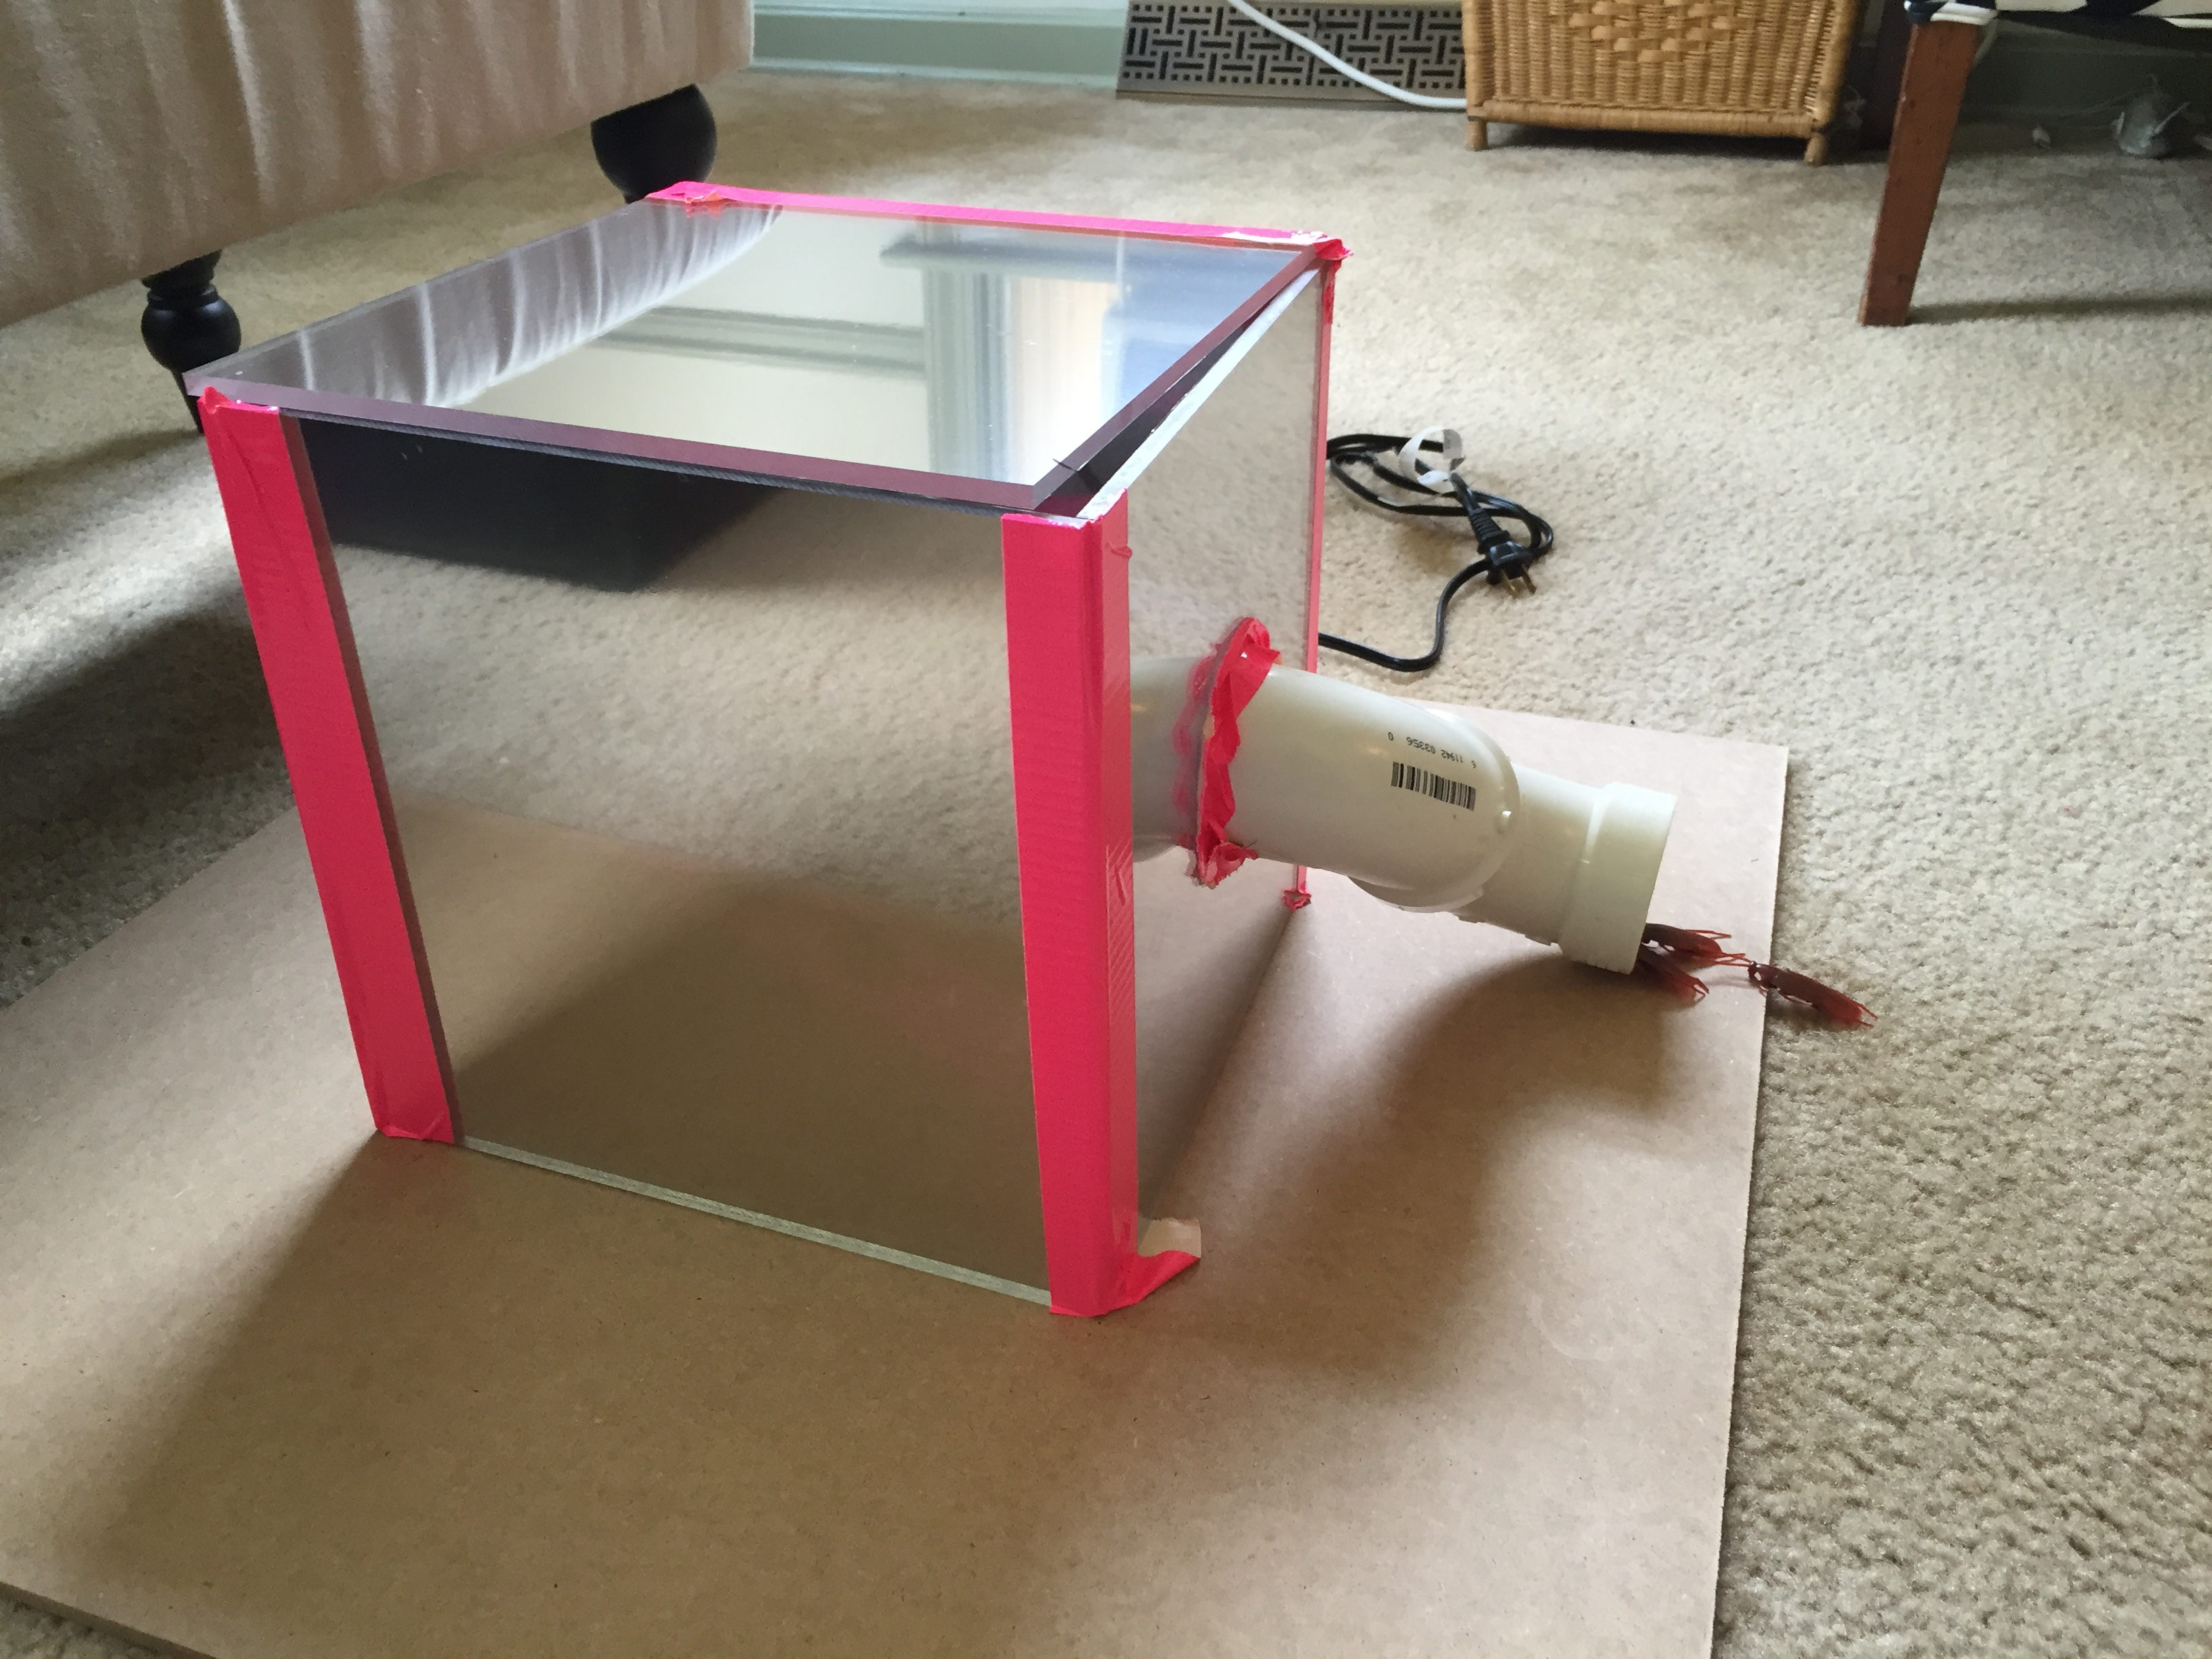
\includegraphics[height=0.75\textheight]{IMG_5941}
 \end{center}
 \end{block}
\end{frame}

\begin{frame}{Do you want to start your own Makerspace?}
 \begin{block}{Budget for equipment}
  \begin{itemize}
   \item Around \$20k in major equipment such as 3D printers (\$2.5k/ea), laser cutter (\$5k), thermoformer (\$5k), CNC cutter (\$7k)
   \item Electronics base equipment: oscilloscopes, function generators, soldering stations (\$5k)
  \end{itemize}
 \end{block}
 \begin{block}{Space requirements}
  \begin{itemize}
   \item Constraints due to local regulations
   \item Venting for 3D printers and laser cutter
  \end{itemize}
 \end{block}
 \begin{block}{Annual budget for personnel and projects}
  \begin{itemize}
   \item \$2k per semester for student project support
   \item Undergraduate and graduate TA support in kind
  \end{itemize}
 \end{block}
\end{frame}

\begin{frame}{Summary}
 \begin{block}{Small Hall Makerspace at W\&M}
  \begin{itemize}
   \item The majority of physics students will enter a career that will require them to work on projects that are more similar to makerspace activities than to solving homework problems: we should provide them with the experiences to be successful in these projects.
   \item At a liberal arts institution with no natural engineering home for prototyping and entrepreneurship, physics departments are uniquely placed to benefit with minimal cost from the possibilities that the maker movement allows.
  \end{itemize}
 \end{block}
\end{frame}

\end{document}
